\section{Theoretische Grundlagen}
\label{sec:theoretGrundl}
Dieses Kapitel behandelt die theoretischen Grundlagen für verwendete Verfahren, Hardware und Software. Es hat die Aufgabe den Leser:innen für das Verständnis essentielle Informationen zu übermitteln.
\subsection{Globales Positionsbestimmungssystem}
\label{subsec:tGPS}
%TODO rewrite this
\glqq GPS ist ein satellitengestütztes Navigationssystem mit 32 aktiven Satelliten (Stand: 2014) und heißt vollständig "Navigational Satellite Timing and Ranging - Global Positioning System" (NAVSTAR-GPS). Das Verteidigungsministerium der USA (Department of Defense, DOD) ist der Betreiber von GPS und hat es hauptsächlich für militärische Zwecke vorgesehen. GPS wurde am 17. Juli 1995 offiziell in Betrieb genommen.

Mit GPS lässt sich der Standort und die Zeit ermitteln. Die Standortbestimmung umfasst die geographische Länge und Breite, sowie die Höhe. Die Genauigkeit liegt zwischen 13 Meter und 1 Millimeter. Genauigkeiten unter 2 Meter sind nur mit viel Aufwand (Differential-GPS) erreichbar. Übliche GPS-Empfänger und Handys haben eine Genauigkeit von 13 bis 2 Meter. Die horizontale Genauigkeit liegt bei 10 bis 15 Meter.
Drei Satelliten werden benötigt, um Längen-, Breitengrad und Höhe errechnen zu können. Der vierte Satellit wird benötigt, um die Uhr des Empfängers mit den Uhren der Satelliten synchronisieren zu können. Die Zeiten müssen absolut übereinstimmen, sonst kommt es zur Fehlberechnung.
Einfach ausgedrückt, wird aus der Laufzeit des Signals vom Satelliten die Entfernung zum Satelliten vom Empfänger errechnet. In Kombination mit mehreren Satelliten kann man die Position auf der Erdoberfläche bestimmen (Triangulation).\grqq \ 
(\cite{schnabelGPS})

\subsection{Inertiale Messeinheit}
\label{subsec:tIMU}
Eine \ac{IMU} z. Dt. inertiale Messeinheit kombiniert mehrere verschiedene Sensoren zur Bestimmung von Lage, Beschleunigungen und Position im dreidimensionalen Raum. Um eine zuverlässige Ermittlung dieser Werte zu gewährleisten, werden Beschleunigungsmessung, Rotationsgeschwindigkeitsmessung (und in einigen Fällen auch die Messung des Magnetfeldes der Erde) kombiniert. Inertiale Messeinheiten werden unter anderem für die Navigation von Flugzeugen, Raumschiffen und Schiffen verwendet. In der Automobilindustrie werden \ac{IMU}s verwendet, um das Fahrverhalten von Autos zu bestimmen und dieses zu verbessern.\\
Die \ac{IMU} liefert die Beschleunigungen sowohl in x-, y- als auch z-Richtung, die Winkelgeschwindigkeiten um die x-, y- als auch z-Achse (und in manchen Fällen die magnetische Feldstärke in x-, y- als auch z-Richtung). Um die Lage zu bestimmen können die Beschleunigungssensoren verwendet werden, indem die Lage der Erdbeschleunigung im dreidimensionalen Raum ermittelt wird, dies funktioniert allerdings nur, solange der Sensor sich in Ruhelage befindet. Alternativ können die Rotationsgeschwindigkeiten integriert werden, dies ergibt aber aufgrund von Messfehlern nach einiger Zeit Abweichungen (drift).\\ Um eine fehlerfreie Ermittlung der Lage zu ermöglichen kann Sensorfusion betrieben werden. Darunter versteht man einen Prozess, der Signale von zwei oder mehr Sensoren zusammenfasst. Im Falle einer \ac{IMU} kann die Ermittlung mittels Accelerometern, Gyroskopen und Magnetometern wie in Sektion \ref{subsec:IMUprogram} beschrieben kombiniert werden.
(\cite{UCAM-CL-TR-696})

\subsection{Raspberry Pi Zero 2 W}
\label{subsec:RasPi}
Der Raspberry Pi Zero 2 W ist ein Einplatinencomputer der Raspberry Pi Foundation. Mit einem 1GHz quad-core 64-bit Arm Prozessor, 512MB SDRAM, eingebauten WLAN- und Bluetooth-Modulen und 40 pins für GPIO, SPI, I2C, UART und Spannungsversorgung stellt er ein Umfangreiches Paket für die Interaktion mit diverser Sensorik dar. Als Betriebssystem bietet die Raspberry Pi Foundation eine auf Debian basierte Linux-Distribution namens Raspberry Pi OS an. Raspberry Pi OS ist in drei verschiedenen Varianten verfügbar, diese unterscheiden sich im Funktionsumfang und der Installationsgröße. Aufgrund der limitierten Rechenleistung des \ac{Raspi} Zero 2 W und der fehlenden Notwendigkeit für eine Desktop-Umgebung ist die Lite-Version am besten geeignet.
\begin{figure}[h]
\centering
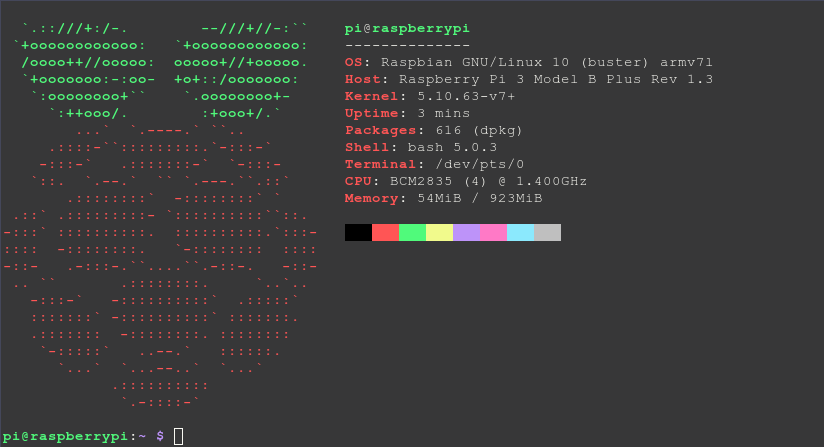
\includegraphics[scale=0.6]{pineofetch.png}
\caption{Das Commandline-Tool neofetch am \ac{Raspi} Zero 2 W}
\label{fig:pineofetch}
\end{figure}

\subsection{Python}
\label{subsec:tPython}
Python ist eine in den frühen 1990ern von Guido van Rossum erstellte Programmiersprache. Heutzutage zeichnet sich Python dadurch aus, dass es quelloffen und für jeden nutzbar ist. Außerdem nimmt Python dem Programmierenden durch die im Vergleich zu Sprachen wie C++ einfache Syntax und das integrierte Ressourcenmanagement viel Arbeit ab. Ein Nachteil von Python ist, dass es im Vergleich mit anderen Sprache wie C++ eine sehr langsame Programmiersprache ist. Aufgrund seiner Simplizität und Verfügbarkeit für Plattformen wie Microsoft Windows, macOS, Linux und FreeBSD gibt es sehr viele quelloffene Bibliotheken für Python, was das Programmieren noch weiter erleichtert. Ein weiterer Unterschied zu Sprachen wie C, C++ oder Rust besteht darin, dass Python interpretiert statt kompiliert wird. Dies hat zur Folge, dass der Code direkt ausgeführt werden kann, solange ein geeigneter Python-Interpreter und die verwendeten Bibliotheken installiert sind, ohne zuvor für jede Plattform eigens kompiliert werden zu müssen.
(\cite{matthes-2019})

\subsection{Qt}
\label{subsec:tQt}
Qt ist eine von der Qt Company entwickelte Bibliothek für die Entwicklung von grafischen Oberflächen. Sie ist wie Python plattformübergreifend und unterstützt unter anderem Microsoft Windows, macOS, Unixartige Betriebssysteme mit X11, Linux mit Wayland, Android und iOS. Qt unterstützt ebenfalls die Entwicklung mit verschiedenen Programmiersprachen, darunter Python, C++ und Qt QML, zusätzlich wird Unterstützung für Rust und Go von der Qt-Community angeboten. Qt ist wie Python Quelloffen und kann für die Open-Source-Programmierung frei verwendet werden. Die neueste Qt-Python Bibliothek heißt PySide6, mit nur fünf Zeilen Python-Code kann ein leeres Fenster erstellt werden.
\begin{figure}[h]
\centering
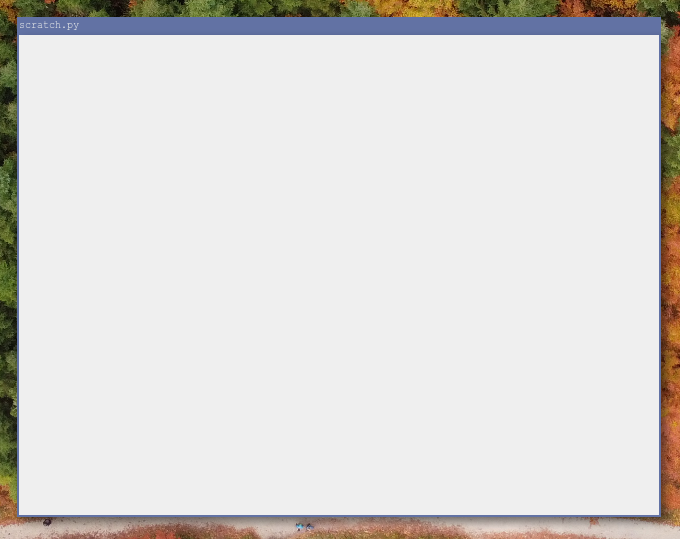
\includegraphics[scale=0.5]{EmptyQtWindow.png}
\caption{Leeres PySide6-Fenster auf Linux unter X11}
\label{fig:EmptyQtWindow}
\end{figure}